\documentclass[a4paper]{report}

% Input format
\usepackage[utf8]{inputenc}
\usepackage[english]{babel}

% Page setup
\usepackage[a4paper,margin=2.5cm]{geometry}

% Fonts and typography
\usepackage[T1]{fontenc}
\usepackage{libertine}
\usepackage[tracking,kerning,spacing]{microtype}

% Drawings
\usepackage{tikz}
\usepackage{tikz-uml}

\title{Everything Is Connected: Architecture}
\author{Multimedia Lab — {\scshape ibbt} / Ghent University}
\date{}

\begin{document}
\maketitle

\chapter{{\scshape uml} diagrams}
\section{Client}
\begin{tikzpicture}
  \umlclass[x=0,y=0]{SlidePresenter}{
      generator : SlideGenerator\\
    }{
      start() : void\\
    }
  \umlclass[x=6,y=0]{SlideGenerator}{
    }{
      init() : void\\
      hasNext() : bool\\
      next() : Slide\\
    }
  \umlclass[x=11,y=0]{Slide}{
      \$element : jQuery\\
      start : function\\
      stop : function\\
      started : Event\\
      stopped : Event\\
      duration : int\\
  }{}
  \umlclass[x=1,y=-4]{CombinedSlideGenerator}{
      generators : SlideGenerator[]
    }{
      addGenerator(Generator) : void\\
    }
  \umlclass[x=6,y=-4]{TitleSlideGenerator}{
      topic : Topic\\
    }{}
  \umlclass[x=11,y=-4]{TopicSlideGenerator}{
      topic : Topic\\
    }{}
   \umlclass[x=6,y=-7]{Topic}{
      uri : String\\
      type : String\\
      label : String\\
   }{}

  \umluniaggreg[mult1=1,mult2=1]{SlidePresenter}{SlideGenerator}
  \umlunicompo[mult1=*,mult2=1]{SlideGenerator}{Slide}
  \umlinherit[geometry=|-|]{CombinedSlideGenerator}{SlideGenerator}
  \umlinherit{TitleSlideGenerator}{SlideGenerator}
  \umlinherit[geometry=|-|]{TopicSlideGenerator}{SlideGenerator}
  \umldep[geometry=|-|]{TopicSlideGenerator}{Topic}
  \umldep[]{TitleSlideGenerator}{Topic}
\end{tikzpicture}

\end{document}
